\documentclass[]{article}

\usepackage[pdftex]{graphicx}
\usepackage{amsmath, amsthm, amssymb, amsfonts, amsbsy}
\usepackage{mathtools}
\usepackage{nicefrac}


%opening
\title{Voltage and energy in Charge Redistribution DACs used in SAR ADCs}
\author{Taimur Rabuske}

\newcommand{\figref}[1]{Figure \ref{#1}}
%\newcommand{\eqref}[1]{Equation (\ref{#1})}


\newcommand{\vref}{\ensuremath{V_\mathrm{REF}}}

\newcommand{\iref}{\ensuremath{I_\mathrm{REF}}}

\newcommand{\eref}{\ensuremath{E_\mathrm{REF}}}

\newcommand{\edac}{\ensuremath{E_\mathrm{DAC}}}

\newcommand{\vcm}{\ensuremath{V_\mathrm{CM}}}

\newcommand{\vdd}{\ensuremath{V_\mathrm{DD}}}

\newcommand{\cu}{\ensuremath{C_0}}


\newcommand{\cpcu}{\ensuremath{\nicefrac{\cp}{\cu}}}
\newcommand{\dccp}{\ensuremath{\nicefrac{\dcp}{\cp}}}








\begin{document}

\maketitle

\begin{abstract}

This document describes the development of a simplified and a general models for calculation of voltage and energy in capacitive DAC topologies used in Charge Redistribution (CR) Successive Approximation Register(SAR) ADCs.

\end{abstract}


\section{Models for voltage and energy in CR ADCs}

We consider that the comparator inputs present infinite impedance and therefore drain no current from the DAC outputs. Following this assumption, the comparator is removed from the analysis, without compromising the accuracy of the models. Most of the switching schemes use only two voltage levels as reference voltages in the DAC arrangement, namely ground and $\vref$. For these topologies, we may rely on a simplified model to compute the DAC output voltage and the energy. Some other switching schemes, on the other hand, use another intermediate reference voltage, such as $\vcm$. For the latter, we devise a general model that support an arbitrary number of references and concurrent switching of multiple capacitors.

\section{Simplified voltage model for CR DACs}
\label{subsec:model_simple}

\label{sec:dac_model}

\begin{figure}
	\centering
	\includegraphics[scale=1.0]{figures/capacitor_switch}
	\caption{Circuit representation of a CR DAC transistioning between abitrary states.}
	\label{fig:capacitor_switch}
\end{figure}

Since the CR DACs are based on switched capacitors, they do not present static power consumption. Therefore, we are only interested in the power consumtion that takes place in the transistions between states. The circuit in \figref{fig:capacitor_switch} provides a good representation of a CR DAC transistioning between abitrary states. In the diagram, $C_\mathrm{T}$ represents the sum of capacitances that has the bottom plate connected to $\vref$ and remain in this condition during the transistion. The capacitor $C_\mathrm{B}$ represents the sum of capacitances with bottom plates connected to ground that are left unchanged during the transition. The remaining capacitor, $C_\mathrm{X}$, represents the capacitance being switched. The switch $S_1$ is initially connected to ground and is switched to $\vref$ at time $t=0$. All the voltages and currents on the circuit totally settle at time $t_s$. We can discretize the time domain and define $V_\mathrm{X}(0) \equiv V_\mathrm{X}[i-1]$ and $V_\mathrm{X}(t_s) \equiv V_\mathrm{X}[i]$. Since there is no current path for the top plates of the capacitors, the charge at the node $V_\mathrm{X}$ is conserved.
\begin{equation}
	Q_X[0]=Q_X[1]
	\label{eq:q_conservation}
\end{equation}

The equation \eqref{eq:q_conservation} can be rewritten as follows:
\begin{equation}
	C_\mathrm{X} V_\mathrm{X}[i-1] + C_\mathrm{T} \left( V_\mathrm{X}[i-1] -\vref \right) + C_\mathrm{B} V_\mathrm{X}[i-1] = C_\mathrm{X} \left( V_\mathrm{X}[i] -\vref \right) + C_\mathrm{T} \left( V_\mathrm{X}[i] -\vref \right) + C_\mathrm{B} V_\mathrm{X}[i] 
	\label{eq:Q1}
\end{equation}

Solving \eqref{eq:Q1} for $V_\mathrm{X}[i]$ leads to
\begin{equation}
	V_\mathrm{X}[i] = V_\mathrm{X}[i-1]+\frac{C_\mathrm{X}}{C_\mathrm{X}+C_\mathrm{T}+C_\mathrm{B}}\vref.
	\label{eq:V_X}
\end{equation}

Similarly, if $C_\mathrm{X}$ is switched from $\vref$ to ground, \eqref{eq:V_X} becomes
\begin{equation}
	V_\mathrm{X}[i] = V_\mathrm{X}[i-1]-\frac{C_\mathrm{X}}{C_\mathrm{X}+C_\mathrm{T}+C_\mathrm{B}}\vref.
	\label{eq:V_Xgnd}
\end{equation}

%\subsection{Simplified energy model for charge-redistribution DACs}
%\label{subsec:energy_simple}

To quantify the energy consumed from the reference source when $S_1$ switches ground to $\vref$, let us again consider the simple circuit of  \figref{fig:capacitor_switch}, assuming that at the instant $t=0$, $V_\mathrm{X}$ is equal to $V_\mathrm{X}(0)$ and $S_1$ is disconnected from ground and connected to $\vref$. The energy spent to switch the bottom plate of $C_\mathrm{X}$ to $\vref$ is given in \eqref{eq:E_cap}, considering that $\vref$ is a dc voltage source and the current flowing through its terminals is $\iref$.
\begin{equation}
	\eref=\vref \int_0^{t_s} \iref \mathrm \, {d}t
	\label{eq:E_cap}
\end{equation}

The current $\iref$ can be described in terms of the charge drainded to the capacitors connected to $\vref$. This is seen in \eqref{eq:i_dq}, where $Q_{C_\mathrm{X}}$ and $Q_{C_\mathrm{T}}$ are the charges stored in $C_\mathrm{X}$ and $C_\mathrm{T}$, respectively.
\begin{equation}
	\iref(t)=-\left(\frac{\mathrm{d}Q_{C_\mathrm{X}}}{\mathrm{d}t}+\frac{\mathrm{d}Q_{C_\mathrm{T}}}{\mathrm{d}t}\right)
	\label{eq:i_dq}
\end{equation}

Rewriting \eqref{eq:E_cap} in terms of \eqref{eq:i_dq} yields in
\begin{align}
	\eref \left[i\right] &= - \vref \int_0^{t_s} \left(\frac{\mathrm{d}Q_{C_\mathrm{X}}}{\mathrm{d}t}+\frac{\mathrm{d}Q_{C_\mathrm{T}}}{\mathrm{d}t}\right) \mathrm{d}t \\
	&= - \vref \left( \int_{Q_{C_\mathrm{X}}(0)}^{Q_{C_\mathrm{X}}(t_s)} \mathrm{d}Q_{C_\mathrm{X}}  + \int_{Q_{C_\mathrm{T}}(0)}^{Q_{C_\mathrm{T}}(t_s)} \mathrm{d}Q_{C_\mathrm{T}} \right) 
\end{align}

Integrating, we arrive at 
\begin{align}
	\eref\left[i\right] &= -\vref\left[ \left( Q_{C_\mathrm{X}}[i]-Q_{C_\mathrm{X}}[i-1] \right) + \left( Q_{C_\mathrm{T}}[i]-Q_{C_\mathrm{T}}[i-1] \right) \right]\\
	&= -\vref C_\mathrm{X} \left[  \left( V_\mathrm{X}(t_s) -  \vref  \right) - \left( V_\mathrm{X}[i-1] \right)\right] - \vref C_\mathrm{T} \left[ \left( V_\mathrm{X}[i] - \vref \right) -\left( V_\mathrm{X}[i-1] - \vref \right) \right].
	\label{eq:E_q1}
\end{align}
Solving \eqref{eq:E_q1} leads to
\begin{equation}
	\eref \left[i\right]=\vref C_\mathrm{X} \left( \vref + V_\mathrm{X}[i-1] - V_\mathrm{X}[i]\right) + \vref C_\mathrm{T} \left(V_\mathrm{X}[i-1] - V_\mathrm{X}[i]\right).
	\label{eq:E_sw}
\end{equation}
Plugging \eqref{eq:V_X} into \eqref{eq:E_sw} yields in
\begin{equation}
	\eref \left[i\right]=\frac{C_\mathrm{B} C_\mathrm{X} }{C_\mathrm{B} + C_\mathrm{T} + C_\mathrm{X}} \vref^{2}.
	\label{eq:e_ref}
\end{equation}



Equations \eqref{eq:V_X} and \eqref{eq:e_ref} may be readily used to calculate the top-plate voltage and the energy in the DAC topologies based on the principle of charge redistribution, respectively, if only $\vref$ and ground are employed as references. Additionally, the model is only valid if only one capacitor is switched at each transition. 


\section{General voltage model for CR DACs}

In order to develop a broader model, consider the capacitive array in \figref{fig:capacitor_switch_general}, where the bottom plates of $k$ capacitors are switched at the same time from their initial voltages $V_0[i-1],V_1[i-1]...V_k[i-1]$ to arbitrary voltage levels $V_0[i],V_1[i]...V_k[i]$. Again, the principle of charge conservation holds, and the charge of the $i$-th cycle is the same as the previous cycle:

\begin{figure}
	\centering
	\includegraphics[scale=1.0]{figures/capacitor_switch_general}
	\caption{Circuit used to develop the general voltage model for CR DACs.}
	\label{fig:capacitor_switch_general}
\end{figure}

\begin{equation}
	Q_X[i]=Q_X[i-1].
	\label{eq:q_conservation_general}
\end{equation}

By expanding \eqref{eq:q_conservation_general} similarly as in \eqref{eq:q_conservation} and solving for $V_\mathrm{X}[i]$, we arrive at \eqref{eq:vx_general}.

\begin{align}
	V_\mathrm{X}[i] = \frac{
		C_{0} \left( V_{0}[i] - V_{0}[i-1] + V_\mathrm{X}[i-1]\right) + \ldots +
		%C_{1} \left( V_{1}[i] - V_{1}[i-1] + V_\mathrm{X}[i-1]\right) + 
		C_{k} \left( V_{k}[i] - V_{k}[i-1] + V_\mathrm{X}[i-1]\right)}
	{C_{0} + C_{1} + \ldots + C_{k}}
	\label{eq:vx_general}
\end{align}

By collecting the similar terms together, \eqref{eq:vx_general} may be rewritten as \eqref{eq:vx_final}, wheren $N$ indicates the total number of reference sources employed.

\begin{equation}
	V_\mathrm{X}[i]=  \dfrac{\displaystyle\sum_{j=0}^{N-1}C_j(V_\mathrm{X}[i-1]+V_j[i]-V_j[i-1]) }{\displaystyle\sum_{j=0}^{N-1} C_j}
	\label{eq:vx_final}
\end{equation}

%\subsection{General energy model for charge-redistribution DACs}
%\label{sec:sectiona}

In order to compute the energy, we assume that the only voltage levels allowed on the bottom plates of the capacitors are the reference voltages. This simplification does not pose any limitation on the analysis, as this happens naturally in a charge-redistribution DAC. These voltages may comprehend any finite number of voltage sources $V_\mathrm{REF0}, V_\mathrm{REF1}...V_{\mathrm{REF},k}$, even though practical implementations of charge-redistribution DACs use 2 or 3 (i.e. $\vdd$, ground and the common-mode voltage $\vcm$). In the model for voltage in the DAC, we considered that the capacitances are fixed and that the voltages on their bottom plates vary in time. On the other hand, for the energy model, we will use the assumption of fixed and known voltage levels and compute the variation of the capacitance connected to each one of those voltage sources. This analogy is depicted in \figref{fig:capacitor_switch_general_energy} and simplifies the calculation of energy when multiple references or capacitors are switched concurrently. Also, this change of standpoint is not harmful to the analysis because we care most about the amount of energy that is spent from $\vref$, and have limited interest on the distribution of currents among the capacitors.

\begin{figure}
	\centering
	\includegraphics[scale=1.0]{figures/capacitor_switch_general_energy}
	\caption{Circuit used to develop the general energy model for CR DACs.}
	\label{fig:capacitor_switch_general_energy}
\end{figure}

For every state transistion in the DAC, the capacitance connected to a given voltage source $V_{\mathrm{REF},j}$ can be split up into 2 components: $C_{j,\mathrm{s}}$, which is the capacitance that was maintained static since the previous cycle; and $C_{j,\mathrm{d}}$, which is the capacitance that was just connected to the reference voltage in the current cycle. Additionally, $C_{j,\mathrm{d}}$ is further subdivided according to the voltage that was previously applied to the bottom plate of these capacitors, so that $C_{j,\mathrm{d}1}$ corresponds to all the capacitors previously connected to $V_\mathrm{REF1}$, $C_{j,\mathrm{d}2}$ corresponds to all the capacitors previously connected to $V_\mathrm{REF2}$ and so on. Note that if a capacitor is disconnected from the voltage source in the transition of states, it does not contribute to its energy consumption. The assignment of capacitance values is exemplified for $V_\mathrm{REF0}$ in \figref{fig:capacitor_a}.

\begin{figure}
	\centering
	\includegraphics[scale=1.0]{figures/capacitor_a}
	\caption{Example of capacitance values assignment for $V_\mathrm{REF0}$.}
	\label{fig:capacitor_a}
\end{figure}


At each cycle, the energy drawn from $V_{\mathrm{REF},j}$ is the sum of the energies spent to charge $C_{j,\mathrm{s}}$ and $C_{j,\mathrm{d}0},C_{j,\mathrm{d}1}...C_{j,\mathrm{d},k}$. Thus, the energy consumed in the $i$-th cycle is given by:

\begin{equation}
	E_{\mathrm{REF},j}[i] = E_{j,\mathrm{s}}[i]+\sum\limits_{k=0}^{N-1}E_{j,\mathrm{d},k}[i]
	\label{eq:ej}
\end{equation}

Following a similar reasoning to that presented in Section \ref{subsec:model_simple}, \eqref{eq:ej} may be rewritten as
\begin{equation}
	E_{\mathrm{REF},j}[i] = - V_{\mathrm{REF},j} \left(
	\int_{Q_{C_{j,\mathrm{s}}}[i-1]}^{Q_{C_{j,s}}[i]} \mathrm{d}Q_{C_{j,s}}  +
	\sum\limits_{k=0}^{N-1}\int_{Q_{C_{j,\mathrm{d},k}}[i-1]}^{Q_{C_{j,\mathrm{d},k}}[i]} \mathrm{d}Q_{C_{j,\mathrm{d},k}}
	\right).
\end{equation}

%\begin{equation}
%\begin{split}
%E_{REFj}[i] = 
%\frac{1}{C_{D0[i]} + C_{D1[i]} + C_{D2[i]} + C_{S[i]}} \\
%\cdot \left[ - C_{D0[i]} V_{D0[i-1]} - C_{D1[i]} V_{D1[i-1]} - C_{D2[i]} V_{D2[i-1]} \right.\\
%\left. + V_{X[i-1]} \left(C_{D0[i]} + C_{D1[i]} + C_{D2[i]} + C_{S[i-1]}\right) \right.\\
%\left. + \vref \left(C_{D0[i]} + C_{D1[i]} + C_{D2[i]} - C_{S[i-1]} + C_{S[i]}\right) \right]
%\end{split}
%\end{equation}

By solving and simplifying, we arrive at 
\begin{equation}
	E_{\mathrm{REF},j}[i] = 
	- V_{\mathrm{REF},j} \left( C_{j,\mathrm{s}} \left(V_\mathrm{X}[i-1]-V_\mathrm{X}[i]\right) + 
	\sum\limits_{k=0}^{N-1}C_{j,\mathrm{d},k} \left( V_{j,\mathrm{d},k}[i-1] + V_\mathrm{X}[i]- V_\mathrm{X}[i-1] -V_{\mathrm{REF},j} \right)
	\right)
	\label{eq:e_final}
\end{equation}

The total energy consumed during a transition is found summing the contribution of all the reference sources.
\begin{equation}
	E_\mathrm{total}=\sum\limits_{j=0}^{N-1}E_{\mathrm{REF},j}
	\label{eq:e_total}
\end{equation}

Therefore, \eqref{eq:vx_final}, \eqref{eq:e_final} and \eqref{eq:e_total} can be employed in order to find the total energy consumption and the contribution of all the reference sources in the ADC.  

The general model requires solving slightly more complicated equations than the proposed simplified model to compute the energy of switching schemes. On the other hand, this general model is easier to be implemented algorithmically on a computer, which makes it a good alternative to automate the computations. One of the advantages of automating the calculations is that it makes easier to extend the analysis to new switching schemes as they appear.







\end{document}
